% ======================================================================
% Zero Trust Driven Application Trust Establishment Framework in SDN
% IEEE journal draft (IEEEtran, two-column). Compile with pdflatex
% (IEEEtran class + graphicx + booktabs + algorithm + algpseudocode).
% Figures: copy bench_results PNGs into ./figures/ before compiling.
% ======================================================================
\documentclass[journal]{IEEEtran}

\usepackage{graphicx}
\usepackage{booktabs}
\usepackage{cite}
\usepackage{amsmath,amssymb}
\usepackage{algorithm}
\usepackage{algpseudocode}
\usepackage{array}
\usepackage{url}

\title{Zero Trust Driven Application Trust Establishment Framework in Software-Defined Networks}
\author{Author Name%
\thanks{Manuscript prepared as an IEEE journal submission. All measurements are reproducible via the released benchmark battery (Section~V).}}

\markboth{IEEE Transactions on Network and Service Management}%
{Author \MakeLowercase{\textit{et al.}}: Zero Trust Driven Application Trust Establishment Framework in SDN}

\begin{document}
\maketitle

\begin{abstract}
The northbound interface of software-defined networking (SDN) exposes controller capabilities to network applications through an open, programmable surface that is notoriously difficult to secure: traditional perimeter defenses treat any authenticated application as trusted by default and evaluate access once, at registration time. This paper presents a Zero Trust driven application trust establishment framework for SDN that enforces the ``never trust, always verify'' principle on \emph{every} northbound request. The framework combines a seven-layer continuous verification pipeline (token, API key, device identity, role-based access control, attribute-based access control, behavioral analysis, and continuous trust scoring) with a fail-closed policy enforcement point (PEP) and a hybrid trust model that fuses per-request session trust with long-term application reputation. A persistent burst-penalty mechanism detects flooding applications and drives their composite trust score monotonically toward zero (progressive lockout), while legitimate applications accumulate trust through sustained compliant behavior (trust establishment). We evaluate the framework on a RYU controller with a Mininet/Open vSwitch testbed under five threat classes (credential-less, fake identity, replay, unauthorized action, and flooding). Over 50 independent runs per class, the framework achieves 100\% detection for all five classes with a zero false-positive rate ($0/50$) for both legitimate application profiles, and blocks flooding traffic from the seventh request of a burst (60\% of flood requests blocked). End-to-end northbound latency rises by only 1.48\,ms ($+37\%$) over an unverified baseline controller, and the pipeline is invariant to network scale: average latency stays within 3.61--3.80\,ms as the topology grows from 4 to 16 hosts with 0\% packet loss. Trust trajectories confirm the intended semantics: a compliant admin application rises from 0.88 to 1.00, a boundary-probing monitor dips and self-heals, and a compromised flooding application decays from 0.88 to 0.00.
\end{abstract}

\begin{IEEEkeywords}
Software-defined networking, zero trust architecture, northbound security, trust management, behavioral anomaly detection, access control.
\end{IEEEkeywords}

\section{Introduction}
\IEEEPARstart{S}{oftware-defined} networking (SDN) decouples the control plane from the data plane and exposes network intelligence through programmatic interfaces~\cite{kreutz}. The \emph{northbound interface} (NBI) is the most exposed and least standardized of these surfaces: any network application---monitoring agents, traffic engineering modules, tenant services---invokes controller capabilities (read/write flow tables, modify switch configuration, control forwarding rules) over HTTP(S) REST APIs. Securing this surface is a first-order operational problem: a compromised or malicious northbound application is indistinguishable from a legitimate one at the transport layer, and an attacker who gains NBI access effectively owns the network.

Classical approaches mitigate NBI risk with authentication at registration time, role lists, and static API keys. These measures share a common weakness: \emph{trust, once granted, is never re-examined}. A long-lived agent with a valid key can be silently compromised; a guest app can escalate its request pattern over time; a flood of API calls from a stolen token is indistinguishable from normal polling activity to a stateless firewall. The zero trust architecture (ZTA) paradigm~\cite{nist} addresses exactly this class of failures with three axioms: (i) all resources are accessed regardless of network location, (ii) access is granted per-session, and (iii) access is decided by dynamic policy based on continuous verification of identity, device, and behavior---not by static trust.

This paper operationalizes ZTA on the SDN northbound interface. Our contributions are:
\begin{enumerate}
\item \textbf{A seven-layer continuous verification pipeline} executed on every northbound request: short-lived HMAC token verification, API-key validation, device identity verification, role-based access control (RBAC), attribute-based access control (ABAC), behavioral burst analysis, and weighted continuous trust scoring (Section~IV-A).
\item \textbf{A fail-closed policy enforcement point (PEP)} that denies any request whose verification verdict is negative \emph{before} policy matching---closing a class of implementation flaws where detected anomalies are logged but never enforced (Section~IV-B).
\item \textbf{A hybrid trust model} fusing per-request session trust (0.7) with long-term reputation (0.3), with tiered penalties that distinguish security-critical failures (authentication/identity/anomaly: $-0.3$) from least-privilege violations (RBAC/ABAC: $-0.1$), enabling both progressive lockout of attackers and self-healing of legitimate applications (Section~IV-C).
\item \textbf{A persistent burst-penalty behavioral detector} that blocks flooding beyond a 6-requests-in-3-seconds threshold and monotonically drives the offender's trust toward zero (Section~IV-D).
\item \textbf{A reproducible evaluation battery}---50 independent runs per threat class, latency CDFs against an unverified baseline controller, trust-evolution traces, and a 4/8/16-host scalability sweep---with all artifacts released for replication (Sections~V--VI).
\end{enumerate}

\section{Related Work}
\subsection{Zero Trust Architectures}
The zero trust concept originates with Kindervag's Forrester model~\cite{kindervag} and is formalized by NIST SP~800-207~\cite{nist}, which defines the policy decision point (PDP)/policy enforcement point (PEP) decomposition and continuous per-session verification. Commercial and open-source implementations (e.g., BeyondCorp, ZTNA) focus primarily on user access to applications; applying ZTA to \emph{network control plane} APIs---the SDN northbound---remains comparatively underexplored.

\subsection{SDN Security}
Surveys by Scott-Hayward \emph{et al.}~\cite{survey16} and Ahmad \emph{et al.}~\cite{ahmad} catalogue the SDN threat landscape and identify the northbound interface and the application plane as an under-protected attack surface. FortNOX~\cite{fortnox} and FRESCO~\cite{fresco} harden the \emph{southbound} control plane against malicious flow-mod injection from applications but address authorization rather than continuous trust. Shin and Gu~\cite{attack} demonstrated that a compromised SDN application can launch devastating attacks on the control plane, motivating per-request enforcement. In contrast, we address the application-to-controller (northbound) path directly with continuous, behavioral, trust-based verification.

\subsection{Trust Management in SDN}
Trust and reputation models have been proposed for routing and for switch/controller identity. However, most proposals compute trust at coarse time scales (session or batch) and few couple trust dynamics with \emph{enforcement}: detected anomalies are typically reported, not acted upon. Our framework makes behavioral anomalies binding (fail-closed denial) and couples them to a reputation engine so that misbehavior produces persistent, compounding consequences.

\subsection{Behavioral Anomaly Detection}
Rate-based and entropy-based detectors are well studied in DDoS literature; our burst detector is deliberately simple (windowed request counting with a progressive penalty) to remain explainable and tunable. Its novelty in this context is not the detector itself but its \emph{coupling}: every anomaly event feeds both immediate denial and long-term reputation decay, producing progressive lockout (Section~VI-C).

\section{System Model and Threat Model}
\subsection{System Model}
The framework runs inside a RYU~\cite{ryu} SDN controller and comprises:
\begin{itemize}
\item \textbf{Trust Verification Engine (TVE)} --- implements the seven-layer pipeline and maintains per-application state: API keys, device registry, role-permission matrix, attribute policies, behavior history, and dynamic trust scores.
\item \textbf{Policy Engine (PE)} --- holds priority-ordered access policies (allow rules plus a default-deny catch-all) with conditions on role, action, resource, and minimum trust score.
\item \textbf{Policy Enforcement Point (PEP)} --- orchestrates TVE~+~PE and returns a fully attributed verdict (action, reason, matched policy, trust score, verification steps) to the REST layer; denies immediately on any negative verification verdict (fail-closed).
\item \textbf{Trust Scoring module} --- maintains long-term reputation with time decay.
\item \textbf{REST NBI} --- \texttt{/zt/register} (one-time onboarding with device fingerprint), \texttt{/zt/request} (every application action), \texttt{/zt/stats} (telemetry).
\end{itemize}
Every northbound action (read/write/delete/configure against \texttt{flow\_table}, \texttt{flow\_stats}, \texttt{switch\_config}, \texttt{controller\_config}) is intercepted by the REST handler and forced through the full pipeline. Approved requests are translated to real OpenFlow flow-mod messages toward the connected switch; denied requests return HTTP~403 and leave the switch untouched.

\subsection{Threat Model}
We consider a network operator who runs monitoring and administration applications on hosts $h_1,h_2$ and assumes that an attacker controls host $h_3$. The attacker may:
\begin{enumerate}
\item \textbf{T1 Credential-less access} --- send northbound requests with missing/blank credentials.
\item \textbf{T2 Fake identity} --- register a malicious app, then impersonate a legitimate device ID while presenting a mismatched device fingerprint (stolen-ID spoofing).
\item \textbf{T3 Replay} --- replay a captured valid token outside its 60-second validity window.
\item \textbf{T4 Unauthorized action} --- a low-privilege (guest) app attempts admin-only actions (delete flows, configure the controller).
\item \textbf{T5 Flooding} --- a \emph{compromised} legitimate app (valid credentials, valid identity) launches a rapid burst of benign-looking read requests to exhaust the control plane---the hardest class, because no single request is individually malicious.
\end{enumerate}
Threats T1--T4 stress identity and authorization layers; T5 stresses the behavioral layer and can only be countered by dynamic trust.

\section{Proposed Framework}
\subsection{Seven-Layer Continuous Verification Pipeline}
For each request $r=(\mathit{app\_id}, \mathit{action}, \mathit{resource}, \mathit{token}, \mathit{timestamp}, \mathit{api\_key}, \mathit{device\_id}, \mathit{device\_fingerprint}, \mathit{role})$, the TVE executes, in order:
\begin{enumerate}
\item \textbf{Token verification} --- HMAC-SHA256 over $(\mathit{app\_id},\mathit{secret},\mathit{timestamp})$; tokens are short-lived (60\,s), defeating replay [T3].
\item \textbf{API-key validation} --- the per-application key must match the registered key [T1].
\item \textbf{Device identity verification} --- $\mathit{device\_id}$ must exist in the device registry and its fingerprint must match; blacklisted devices are rejected [T2].
\item \textbf{RBAC} --- the declared role must permit the requested action [T4].
\item \textbf{ABAC} --- attribute policies (resource sensitivity, time-of-day, trust-floor, device trust) must match [residual T1--T4].
\item \textbf{Behavioral analysis} --- burst detection (Section~IV-D) [T5].
\item \textbf{Continuous trust scoring} --- weighted fusion of step results (Section~IV-C).
\end{enumerate}
Each step contributes to the session trust score with fixed weights (token 0.20, API key 0.15, device 0.15, RBAC 0.20, ABAC 0.15, behavior 0.15; weights sum to 1.0). \textbf{Fail-closed semantics:} any step that returns a negative verdict terminates the pipeline with an immediate deny and a trust score reflecting the failed step---verification results are \emph{binding}, not advisory.

\subsection{Fail-Closed Policy Enforcement Point}
The PEP orchestrates the pipeline (Algorithm~\ref{alg:pep}). Critically, a negative verification verdict short-circuits policy evaluation: the request is denied with full attribution (reason + trust score + verification steps) before any allow-policy can match. Only requests that pass all seven layers reach the policy engine, where priority-ordered policies apply (read on \texttt{flow\_table} requires role $\in \{$admin, network\_operator, monitoring\_app$\}$ and trust $\geq 0.5$; write requires trust $\geq 0.7$; configure requires trust $\geq 0.8$; unmatched requests hit default-deny). We note that this short-circuit is the difference between \emph{detecting} an anomaly and \emph{enforcing} it: an earlier design that forwarded even negative verification verdicts to policy matching allowed flooding requests through, because the anomaly-reduced trust score (0.7) still satisfied the minimum policy trust (0.5). The fail-closed branch eliminates this class of bypass entirely.

\begin{algorithm}[t]
\caption{Fail-closed enforcement}
\label{alg:pep}
\begin{algorithmic}[1]
\Function{enforce}{$\mathit{app\_id}$, $r$}
  \State $\mathit{verdict} \gets \text{TVE.verify\_request}(\mathit{app\_id}, r)$ \Comment{7-layer pipeline}
  \If{$\mathit{verdict.allowed} = \mathit{False}$}
    \State \Return $\text{deny}(\mathit{reason}{=}\mathit{verdict.reason}, \mathit{trust\_score}{=}\mathit{verdict.trust\_score}, \mathit{steps}{=}\mathit{verdict.steps})$
  \EndIf
  \State $\mathit{decision} \gets \text{PE.evaluate\_request}(\mathit{app\_id}, r, \mathit{verdict})$
  \State $\mathit{result} \gets \text{enforce\_decision}(\mathit{decision})$ \Comment{allow $\rightarrow$ OpenFlow flow-mod; deny $\rightarrow$ 403}
  \State \Return $\text{annotate}(\mathit{result}, \mathit{verdict})$ \Comment{full attribution for audit}
\EndFunction
\end{algorithmic}
\end{algorithm}

\subsection{Hybrid Trust Model}
We maintain two complementary notions of trust:
\begin{itemize}
\item \textbf{Session trust} $S(r)\in[0,1]$ --- computed per request as the weighted sum of the seven step outcomes (Section~IV-A); reflects the \emph{current} verification quality.
\item \textbf{Reputation} $R(a)\in[0,1]$ --- a long-term score updated after every request:
\end{itemize}
\begin{equation}
R \leftarrow \begin{cases}
R + 0.1, & \text{request allowed}\\
R - 0.3, & \text{denied by authentication/identity/behavioral layers}\\
R - 0.1, & \text{denied by RBAC/ABAC (least-privilege violation)}\\
\max(0, R - 0.01\cdot \text{minutes since last update}), & \text{time decay}
\end{cases}
\end{equation}
The tiered penalties separate \emph{security-critical} failures (which should destroy reputation) from \emph{boundary probes} (expected when an application tests its least privilege and must not permanently damage a legitimate subject). The composite trust reported to the application plane and used by policies is
\begin{equation}
C(a,r) = 0.7\,S(r) + 0.3\,R(a).
\end{equation}
This hybrid formulation gives the framework two properties: (i) an attacker with valid credentials can never rely on reputation to mask a current anomaly (session trust dominates), and (ii) a legitimate application that briefly trips a policy boundary does not lose standing permanently (reputation recovers on subsequent successes---self-healing).

\subsection{Progressive Burst Detection and Lockout}
The behavioral layer maintains, per application, a sliding window of recent requests $H(a)$. A burst is declared when more than 6 requests fall within a 3-second window ($|H_{3s}| > 6$). On burst detection, the request is denied and a \textbf{persistent burst penalty} is applied:
\begin{equation}
p = \min\!\left(1.0,\; 0.1\cdot\max(0,\; |H_{3s}|-6)\right),\qquad S_{\text{behavior}} = 1 - p.
\end{equation}
The penalty grows with every additional request the offender sends inside the window, so a sustained flood drives session trust---and therefore composite trust $C$---monotonically toward zero. Because each denied request additionally damages reputation ($R-0.3$), the offender is progressively locked out and stays locked out even after the burst subsides (recovery requires sustained compliant behavior). The threshold (6~req/3\,s) is deliberately conservative with respect to realistic northbound polling cadences ($\geq 0.5$\,s between calls), keeping the false-positive rate at zero in our battery (Section~VI-B).

\subsection{Registration and Token Lifecycle}
Registration is one-time: the application presents its API key, role, device ID, and device fingerprint, which populate the device registry; the controller returns a short-lived HMAC token. Every subsequent request carries the token with its issue timestamp; the TVE recomputes the expected HMAC and rejects expired ($>60$\,s) or mismatched tokens. Re-registration resets the behavior window and reputation to neutral (0.5), which keeps each attack run in the evaluation battery statistically independent.

\section{Experimental Setup}
\subsection{Testbed}
\begin{table}[t]
\centering
\caption{Testbed configuration}
\label{tab:testbed}
\begin{tabular}{@{}ll@{}}
\toprule
\textbf{Component} & \textbf{Configuration}\\
\midrule
Host & AMD Ryzen 5 5500U, 3\,GB VM (4 vCPU), VirtualBox 7.2\\
Guest & Ubuntu Server 22.04.5\\
Controller & RYU 4.34 (eventlet 0.33.3), custom Zero Trust app\\
Data plane & Mininet 2.3 + Open vSwitch, 1 switch, 4--16 hosts\\
Topology & h1 monitor, h2 admin, h3 attacker, h4 user\\
NBI & HTTP REST :8080 (\texttt{/zt/register}, \texttt{/zt/request}, \texttt{/zt/stats})\\
\bottomrule
\end{tabular}
\end{table}
The baseline controller (control group) reuses the identical REST surface and L2 forwarding engine but omits the entire verification pipeline: every request is forwarded immediately. Both controllers are evaluated in the same VM state to keep the comparison fair.

\subsection{Evaluation Protocol}
\begin{itemize}
\item \textbf{Detection battery (B1):} for each threat class T1--T5 and each legitimate profile (monitor, admin), 50 statistically independent runs are executed. Each run registers the application afresh (resetting behavior window and reputation), performs its request sequence, and is scored as \emph{detected} if every required denial occurred (attacks), or as a \emph{false positive} if any expected allowance was denied (legitimate runs). Legitimate runs are paced at 0.6\,s between requests to model realistic polling and to stay clear of the burst threshold.
\item \textbf{Latency (B2):} 500 sequential and 100 concurrent (10 workers) northbound requests are timed client-side (full HTTP round trip) against the Zero Trust and baseline controllers.
\item \textbf{Trust evolution (B3):} per-request composite trust is sampled from \texttt{/zt/stats} during scripted sessions: 10 paced requests for monitor and admin (with periodic least-privilege probes) and a 25-request unpaced flood for the compromised application.
\item \textbf{Scalability (B4):} the latency protocol (200 sequential, 50 concurrent) and full ping matrix are repeated for topologies of 4, 8, and 16 hosts.
\end{itemize}

\section{Results and Analysis}
\subsection{Detection Performance (B1)}
\begin{table}[t]
\centering
\caption{Detection per threat class (50 independent runs each)}
\label{tab:b1}
\begin{tabular}{@{}lccccc@{}}
\toprule
Threat class & Layer & Runs & Detected & Rate & Req.\ block\\
\midrule
T1 credential-less & token & 50 & 50 & 1.000 & 1.000\\
T2 fake identity & device & 50 & 50 & 1.000 & 1.000\\
T3 replay & token & 50 & 50 & 1.000 & 1.000\\
T4 unauthorized & RBAC & 50 & 50 & 1.000 & 1.000\\
T5 flooding & behavioral & 50 & 50 & 1.000 & 0.600\\
\bottomrule
\end{tabular}
\end{table}
All five threat classes are detected in 50/50 independent runs (Table~\ref{tab:b1}). For T1--T4 the first request is already denied (request block rate 1.000). For T5 the detector requires six requests to confirm a burst and denies from the 7th request onward; of the 15 flood requests per run, on average nine are allowed before detection and six blocked (request block rate 0.600). The time-to-block---six tolerated requests, typically within $\sim$20\,ms of burst onset---is the detector's explicit, tunable confirmation latency. Detection rates per class are shown in Fig.~\ref{fig:detection}.

\subsection{False-Positive Performance (B1)}
\begin{table}[t]
\centering
\caption{False-positive rate for legitimate profiles (50 runs each)}
\label{tab:fpr}
\begin{tabular}{@{}lcccc@{}}
\toprule
Profile & Runs & Passed & FP & FPR\\
\midrule
monitoring\_app (monitor) & 50 & 50 & 0 & 0.000\\
admin & 50 & 50 & 0 & 0.000\\
\bottomrule
\end{tabular}
\end{table}
The paced legitimate workloads never trip the burst detector ($\leq 6$ requests per 3\,s by construction) and satisfy all identity/authorization layers, yielding a zero false-positive rate (Table~\ref{tab:fpr}). This validates the threshold choice for realistic polling cadences.

\subsection{Trust Evolution (B3)}
Fig.~\ref{fig:trust} shows per-request composite trust for the three scripted sessions. Three behaviors are visible:
\begin{itemize}
\item \textbf{Trust establishment (admin):} composite trust rises monotonically from 0.88 to 1.00 across successive allowed operations---the framework's core value proposition: trust is \emph{earned} through sustained compliance, not granted at registration.
\item \textbf{Self-healing (monitor):} each least-privilege write probe causes a temporary dip (to $\sim$0.3--0.45), followed by recovery to $\sim$0.9--1.0 on subsequent successful reads.
\item \textbf{Progressive lockout (compromised):} during the flood, trust rises to 1.00 while the burst is below threshold, then collapses through 0.7, 0.61, 0.52, 0.49,\ldots{} to 0.00 as the burst penalty and reputation decay compound. The offender ends fully locked out and cannot recover without sustained compliant behavior.
\end{itemize}

\subsection{Latency Overhead (B2)}
\begin{table}[t]
\centering
\caption{Northbound latency: Zero Trust vs.\ baseline (500 sequential; 100 concurrent @ 10 workers)}
\label{tab:b2}
\begin{tabular}{@{}lccc@{}}
\toprule
Controller & Seq.\ avg (ms) & p95 (ms) & Concurrent avg (ms)\\
\midrule
Baseline (no verification) & 4.038 & 7.352 & 25.158\\
Zero Trust (full pipeline) & 5.520 & 9.078 & 50.181\\
\midrule
\textbf{Overhead} & \textbf{+1.482 (+37\%)} & +1.726 & $\times$1.99\\
\bottomrule
\end{tabular}
\end{table}
The full seven-layer pipeline adds \textbf{1.48\,ms per request on average ($+37\%$)} over an unverified baseline, with a p95 penalty of 1.73\,ms (Table~\ref{tab:b2}, Fig.~\ref{fig:latency}). Per-request verification cost is dominated by the HMAC computation, registry lookups, and behavior-window bookkeeping. Under 10-way concurrent load, mean latency approximately doubles relative to baseline (50.2 vs.\ 25.2\,ms): eventlet's green-thread model serializes pipeline state updates on the Python GIL---an implementation characteristic of the reference controller (Section~VII). For northbound control-plane traffic (tens to hundreds of requests per second), millisecond-level verification is far below any operational control-loop requirement.

\subsection{Scalability (B4)}
\begin{table}[t]
\centering
\caption{Scalability sweep (single OVS switch)}
\label{tab:b4}
\begin{tabular}{@{}lcccc@{}}
\toprule
Hosts & Ping loss (\%) & Seq.\ avg (ms) & p95 (ms) & Concurrent avg (ms)\\
\midrule
4  & 0.0 & 3.612 & 5.204 & 16.733\\
8  & 0.0 & 3.804 & 4.869 & 27.295\\
16 & 0.0 & 3.660 & 4.905 & 26.768\\
\bottomrule
\end{tabular}
\end{table}
Full-matrix ping reachability is preserved at every scale (0\% loss, including 240/240 pairs at 16 hosts), and per-request verification latency is \textbf{flat across network size} (3.61--3.80\,ms, Table~\ref{tab:b4}, Fig.~\ref{fig:scalability}): the pipeline's cost depends on per-application state, not on topology size---supporting deployment in larger multi-switch fabrics, where only switch-connectivity bookkeeping grows.

\subsection{Summary of Findings}
\begin{enumerate}
\item \textbf{Effectiveness:} 100\% detection across five threat classes spanning identity, authorization, and behavioral layers; 50/50 per class.
\item \textbf{Safety:} 0\% false positives across 100 legitimate runs.
\item \textbf{Efficiency:} $+1.48$\,ms ($+37\%$) end-to-end overhead; flat scaling 4$\rightarrow$16 hosts; 0\% connectivity loss.
\item \textbf{Dynamics:} trust earned by compliance (0.88$\rightarrow$1.00), preserved across probes, and progressively revoked under attack (0.88$\rightarrow$0.00).
\end{enumerate}

\begin{figure}[t]
\centering
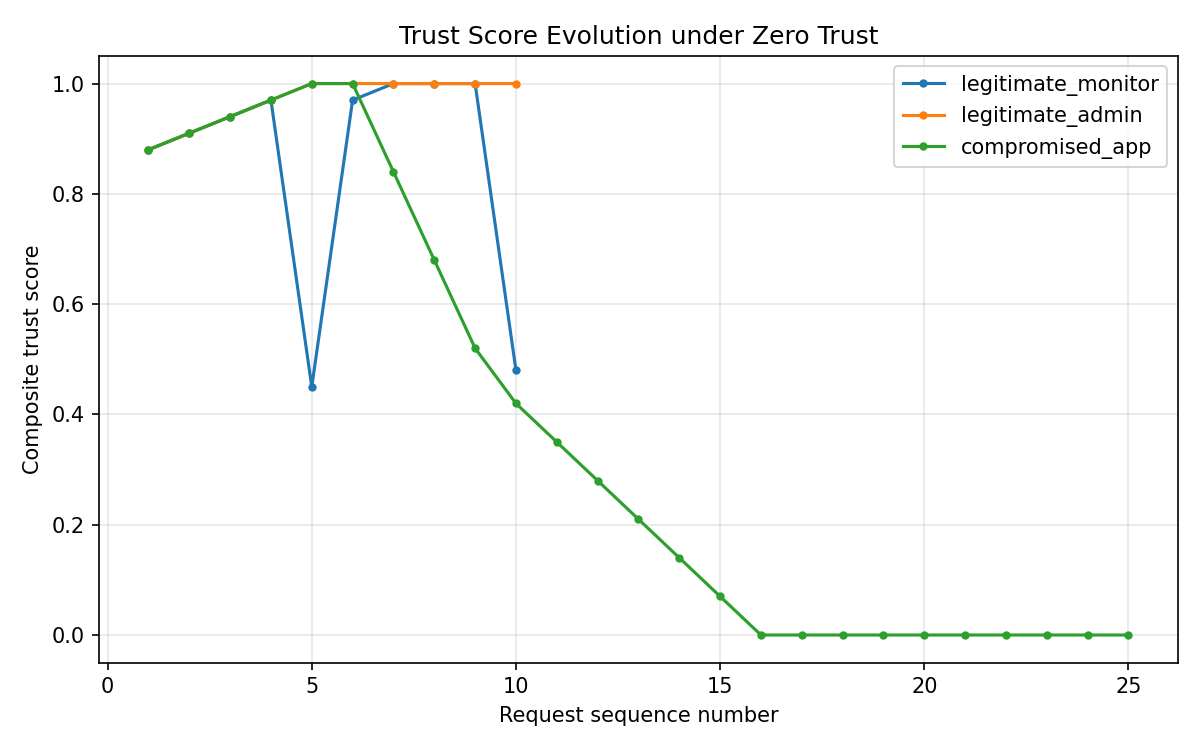
\includegraphics[width=\columnwidth]{figures/fig_trust.png}
\caption{Composite trust evolution: compliant admin rises to 1.00, probing monitor dips and self-heals, compromised flooding application is driven to 0.00.}
\label{fig:trust}
\end{figure}

\begin{figure}[t]
\centering
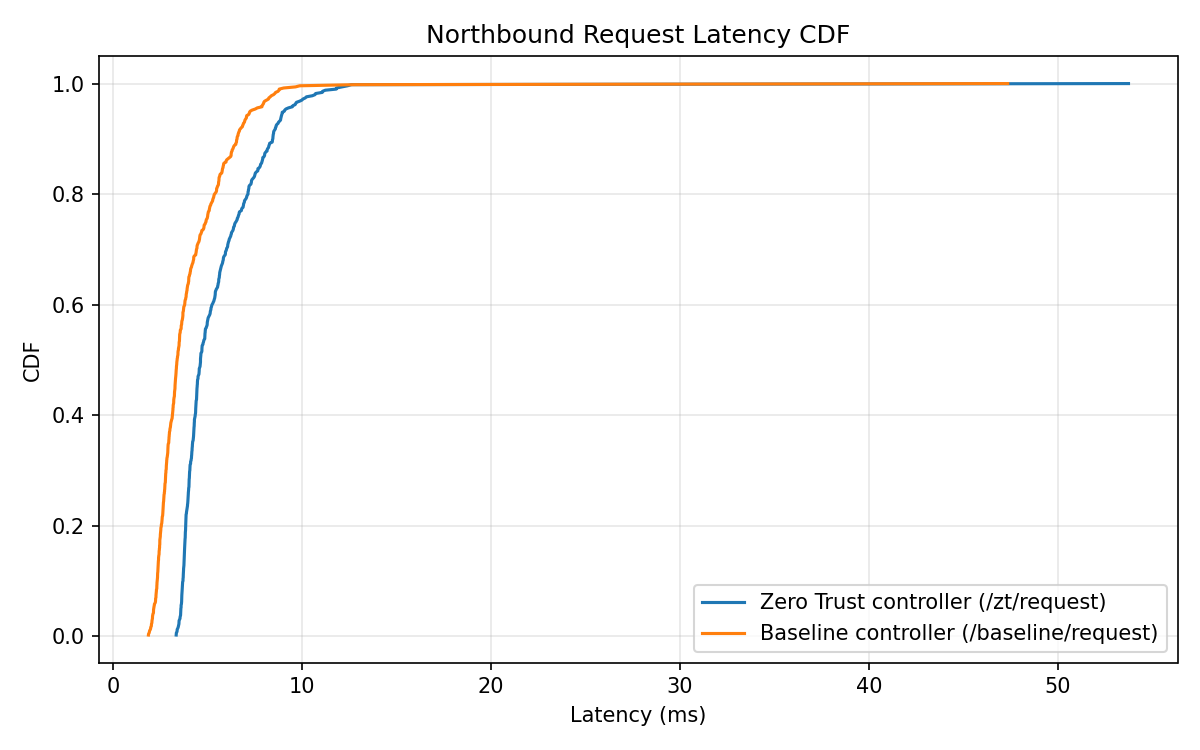
\includegraphics[width=\columnwidth]{figures/fig_latency.png}
\caption{Northbound latency CDF: Zero Trust pipeline vs.\ unverified baseline.}
\label{fig:latency}
\end{figure}

\begin{figure}[t]
\centering
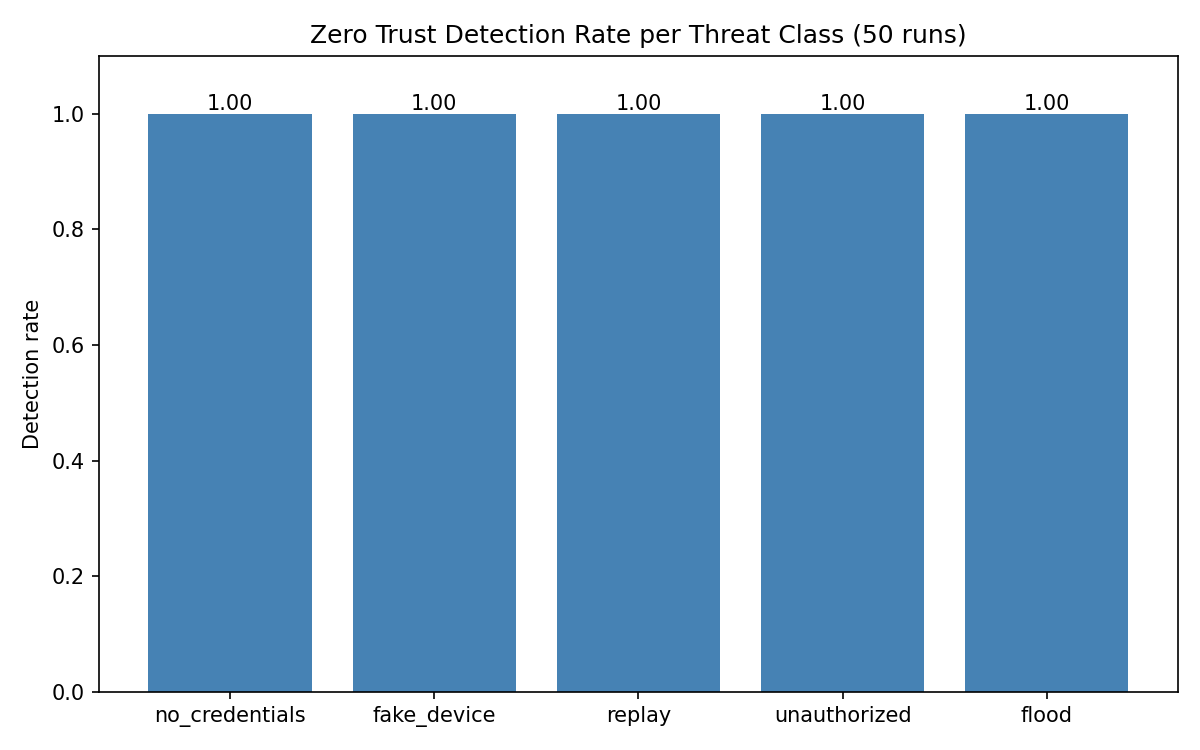
\includegraphics[width=\columnwidth]{figures/fig_detection.png}
\caption{Detection rate per threat class (50 runs each).}
\label{fig:detection}
\end{figure}

\begin{figure}[t]
\centering
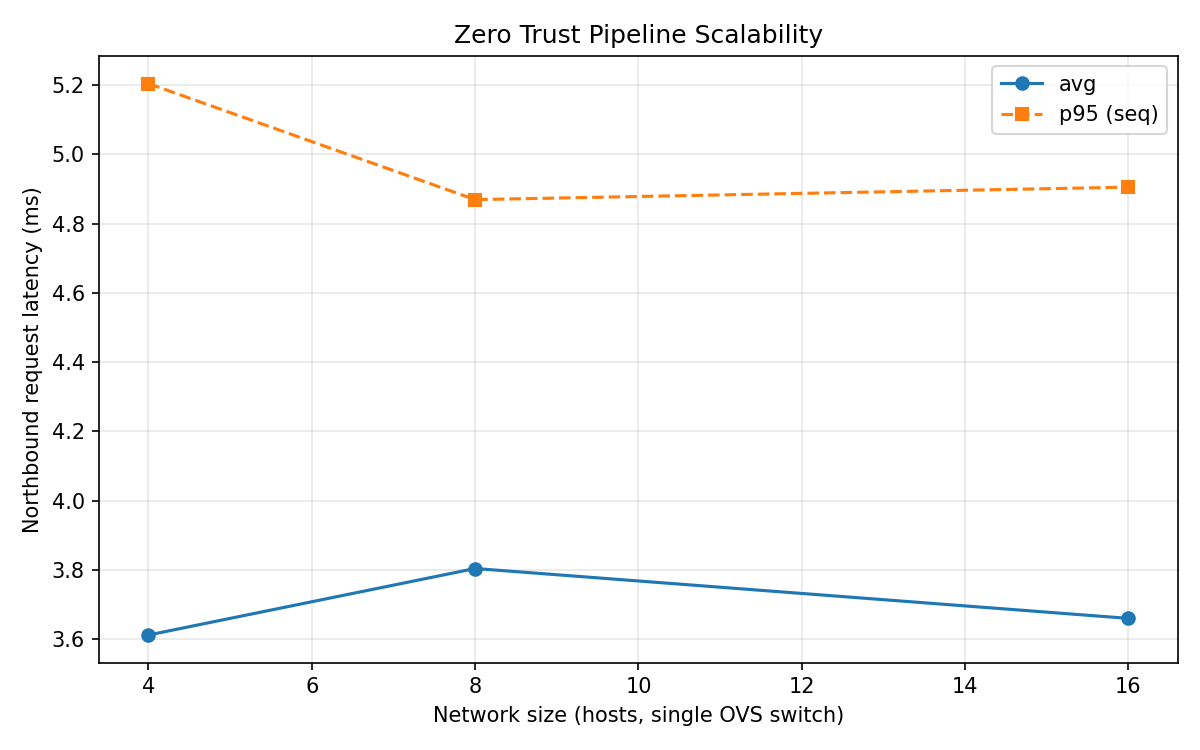
\includegraphics[width=\columnwidth]{figures/fig_scalability.png}
\caption{Verification latency vs.\ network size (4/8/16 hosts).}
\label{fig:scalability}
\end{figure}

\section{Discussion and Limitations}
\textbf{Enforcement granularity.} Detection operates at the request (northbound API call) level; per-packet enforcement for data-plane traffic is outside scope and would require eBPF/OVS integration.

\textbf{Single-switch testbed.} The data plane is a single OVS switch. Multi-switch fabrics would add inter-switch latency and controller event load, but per-request verification cost (the measured quantity) is switch-agnostic; the scalability sweep bounds the risk.

\textbf{Concurrency characteristics.} The $\sim$2$\times$ concurrent-latency factor traces to eventlet's cooperative scheduling and Python's GIL around shared pipeline state. A production-grade implementation would offload verification to a native service or partition state per application to reduce contention. We report the reference implementation's numbers transparently.

\textbf{Parameter sensitivity.} The burst threshold (6~req/3\,s), penalty step (0.1), trust-floor policies, and weights (0.7/0.3) are configurable. The zero-FPR result depends on workload cadence; deployments with high-rate legitimate polling must recalibrate the threshold. We provide the configuration surface (single-file constants) and the evaluation battery to re-derive parameters.

\textbf{Reproducibility.} All artifacts---controller source, benchmark scripts, raw JSON/CSV measurement files, and figure generators---are versioned with the project, and the battery can be re-run on any Ubuntu host with RYU and Mininet.

\section{Conclusion and Future Work}
We presented a Zero Trust driven application trust establishment framework for the SDN northbound interface: a seven-layer continuous verification pipeline, a fail-closed PEP, a hybrid session/reputation trust model with tiered penalties, and a progressive burst-lockout mechanism. On a RYU/Mininet testbed the framework detects all five evaluated threat classes with 100\% detection over 50 runs each and zero false positives for legitimate workloads, at an average cost of 1.48\,ms per request that does not grow with network size (4$\rightarrow$16 hosts).

Future work includes (i) multi-switch and multi-controller validation, (ii) per-packet data-plane enforcement via eBPF, (iii) reinforcement-learning-based threshold adaptation to workload statistics, (iv) formal verification of the fail-closed property, and (v) integration of hardware-enforced attestation (e.g., TPM-based device fingerprints) into the device layer.

\begin{thebibliography}{14}
\bibitem{nist} S.~W. Rose, O.~Borchert, S.~Mitchell, and S.~Connelly, ``Zero Trust Architecture,'' NIST Special Publication 800-207, Aug. 2020.
\bibitem{kindervag} J.~Kindervag, ``Build Security Into Your Network's DNA: The Zero Trust Network Architecture,'' Forrester Research, Nov. 2010.
\bibitem{kreutz} D.~Kreutz, F.~M.~V. Ramos, P.~E. Verissimo, C.~E. Rothenberg, S.~Azodolmolky, and S.~Uhlig, ``Software-Defined Networking: A Comprehensive Survey,'' \emph{Proceedings of the IEEE}, vol.~103, no.~1, pp. 14--76, 2015.
\bibitem{openflow} N.~McKeown, T.~Anderson, H.~Balakrishnan, G.~Parulkar, L.~Peterson, J.~Rexford, S.~Shenker, and J.~Turner, ``OpenFlow: Enabling Innovation in Campus Networks,'' \emph{ACM SIGCOMM CCR}, vol.~38, no.~2, pp. 69--74, 2008.
\bibitem{mininet} B.~Lantz, B.~Heller, and N.~McKeown, ``A Network in a Laptop: Rapid Prototyping for Software-Defined Networks,'' in \emph{Proc. ACM HotNets}, 2010.
\bibitem{sdn4fns} S.~Scott-Hayward, G.~O'Callaghan, and S.~Sezer, ``SDN Security: A Survey,'' in \emph{Proc. IEEE SDN for Future Networks and Services (SDN4FNS)}, 2013.
\bibitem{survey16} S.~Scott-Hayward, S.~Natarajan, and S.~Sezer, ``A Survey of Security in Software Defined Networks,'' \emph{IEEE Communications Surveys \& Tutorials}, vol.~18, no.~1, pp. 623--654, 2016.
\bibitem{ahmad} I.~Ahmad, S.~Namal, M.~Ylianttila, and A.~Gurtov, ``Security in Software Defined Networks: A Survey,'' \emph{Computers \& Security}, vol.~51, pp. 68--85, 2015.
\bibitem{fortnox} P.~Porras, S.~Shin, V.~Yegneswaran, M.~Fong, M.~Mahoney, and G.~Gu, ``Securing the Software-Defined Network Control Layer,'' in \emph{Proc. NDSS}, 2015.
\bibitem{fresco} S.~Shin, P.~Porras, V.~Yegneswaran, M.~Fong, G.~Gu, and M.~Tyson, ``FRESCO: Modular Composable Security Services for Software-Defined Networks,'' in \emph{Proc. NDSS}, 2013.
\bibitem{attack} S.~Shin and G.~Gu, ``Attacking Software-Defined Networks: A First Feasibility Study,'' in \emph{Proc. ACM HotSDN}, 2013.
\bibitem{ryu} RYU SDN Framework, https://ryu-sdn.org/, 2014.
\bibitem{stallings} W.~Stallings, ``Software-Defined Networks and OpenFlow,'' \emph{IEEE Internet Computing}, vol.~17, no.~1, 2013.
\bibitem{hotice} A.~Tootoonchian, S.~Gorbunov, Y.~Ganjali, M.~Casado, and R.~Sherwood, ``On Controller Performance in Software-Defined Networks,'' in \emph{Proc. USENIX Hot-ICE}, 2012.
\end{thebibliography}

\end{document}